\onehalfspacing
An ERGM represents a probability distribution of graphs for a given set, where the probability of observing a graph is dependent on the presence of the various network configurations expressed by the model. Importantly, the unit of analysis in an ERGM is not the number of nodes, but the number of possible ties between all actors in the network ($n(n-1)$). For a binary network, the probability of observing specific network configurations for a given set of actors \(n\) can be expressed as follows: $$ P(X = x) = \frac{\exp \left \{ \theta'z(x)  \right \}}{\kappa (\theta )} $$ where $P(x)$ indicates the probability of a given network, $\theta$ indicates a vector of model parameters, $z(x)$ is a vector of network statistics, and $\kappa$ is a normalising function to ensure a proper probability distribution across a set of random networks \citep{shumate2010exponential}. \medskip 

Network statistics $z(x)$ are counts of the estimated number of configurations in the network, or some function of those counts. The probability of the network depends on how many of those configurations are present and the parameters indicate the importance of each configuration \citep{lusher2013exponential}. Large positive parameters suggest that more configurations of that type are observed in the network than expected by chance alone \citep{robins2009closure}. The following table lists the model parameters used in this thesis and their corresponding network statistic ($z$): \medskip

\begin{sidewaystable}[]
\centering
\caption[Network statistics used in this thesis]{Network statistics used in this thesis*.}
\label{tab:ergm_stats}
\fontdimen16\textfont2=3pt
\fontdimen17\textfont2=3pt
\resizebox{0.9\textwidth}{!}{%	
\begin{threeparttable}
\begin{tabular}{l c l l}
\toprule
Parameter & Graphic & Statistic & Dependences \\ \midrule
Arc (edge) & \begin{minipage}{.12\textwidth} \centering 
\includegraphics[width=0.4\linewidth]{Images/Arc} \end{minipage} & $z_{L} = \sum_{i = 1}^N \sum_{j = 1}^N X_{ij}$ & \\
Reciprocity (mutuality) & \begin{minipage}{.12\textwidth} \centering 
\includegraphics[width=0.4\linewidth]{Images/Reciprocity} \end{minipage} & $z_{\mathit{Reciprocity}} = \sum_{i = 1}^N \sum_{j = 1}^N X_{ij} X_{ji}$ & \\
TwoPath (simple connectivity) & \begin{minipage}{.12\textwidth} \centering 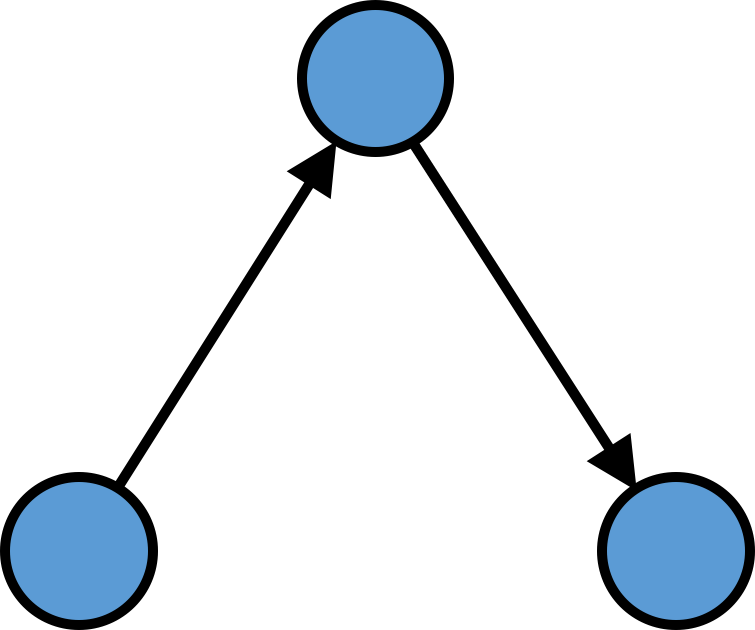
\includegraphics[width=0.4\linewidth]{Images/TwoPath} \end{minipage} & $z_{2P} = \sum_{i \neq j \neq k}^N X_{ij} X_{jk}$ & \\
AinS (popularity spread) & \begin{minipage}{.12\textwidth} \centering 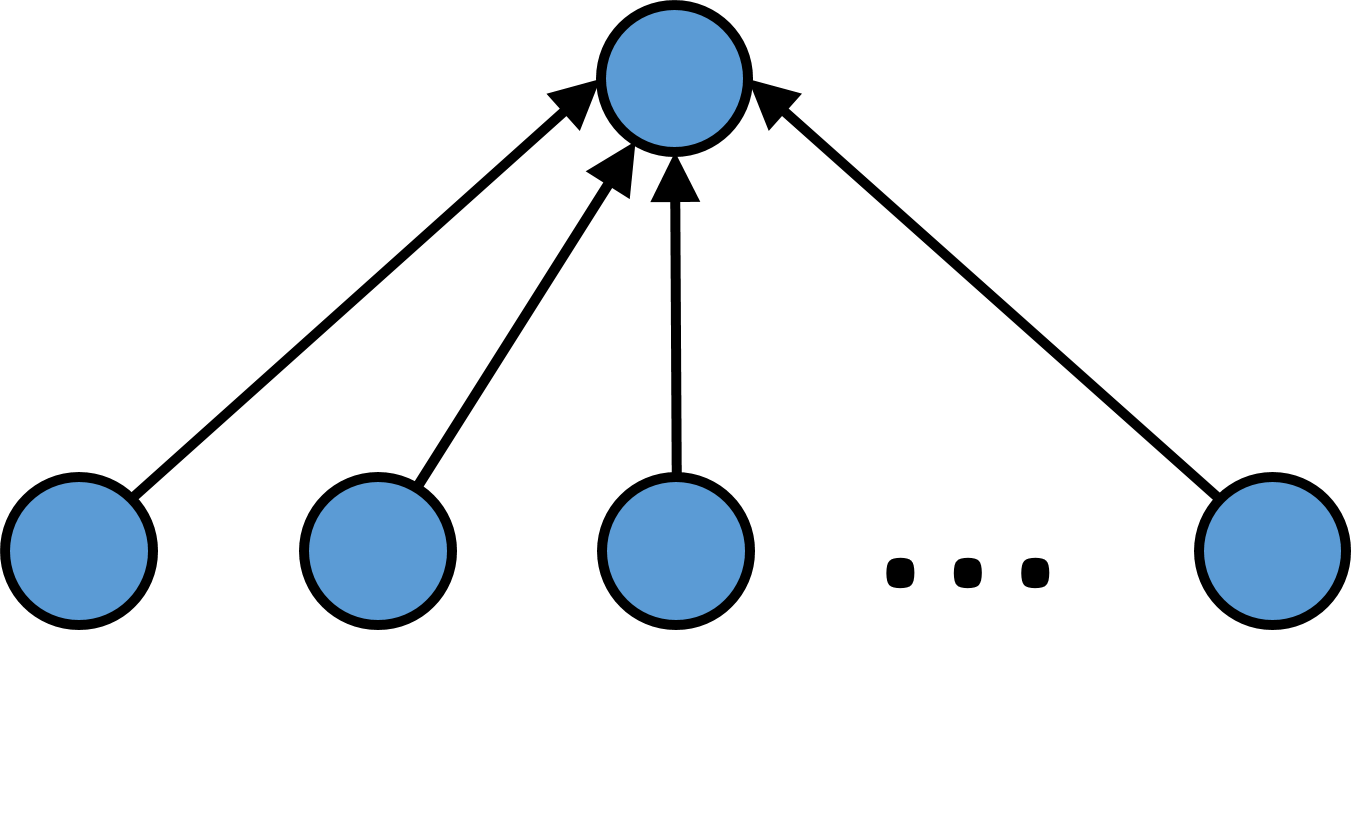
\includegraphics[width=0.6\linewidth]{Images/AinS} \end{minipage} & $z_{AinS} = \sum_{i = 1}^{N-1} \bigg(-1 \bigg)^k \frac{S_k^{in}}{\lambda^{k-2}}$ & \\
AoutS (activity spread) & \begin{minipage}{.12\textwidth} \centering 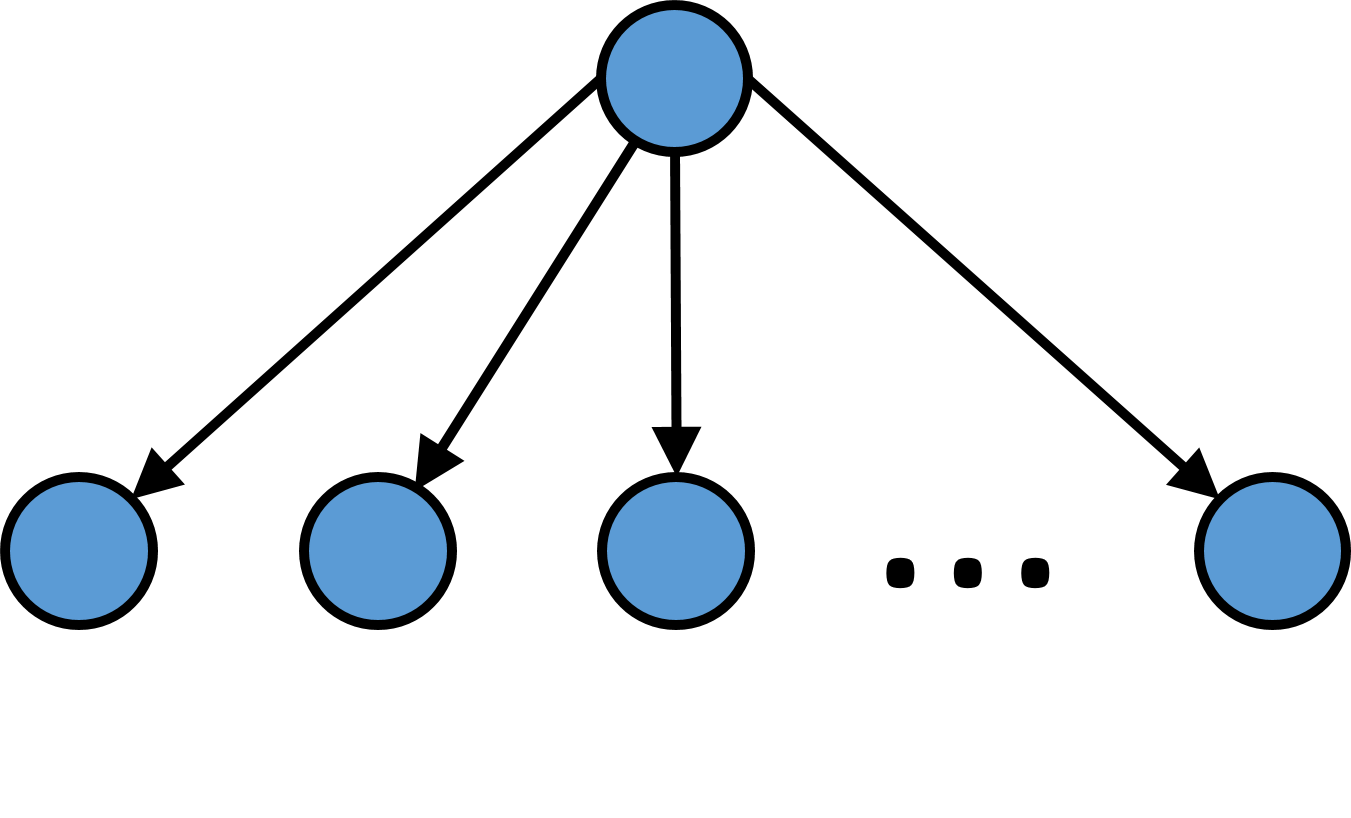
\includegraphics[width=0.6\linewidth]{Images/AoutS} \end{minipage} & $z_{AoutS} = \sum_{i = 1}^{N - 1} \bigg(-1\bigg)^k \frac{S^{Out}_k}{\lambda^{k-2}}$  & \\
AT-T (path closure) & \begin{minipage}{.12\textwidth} \centering 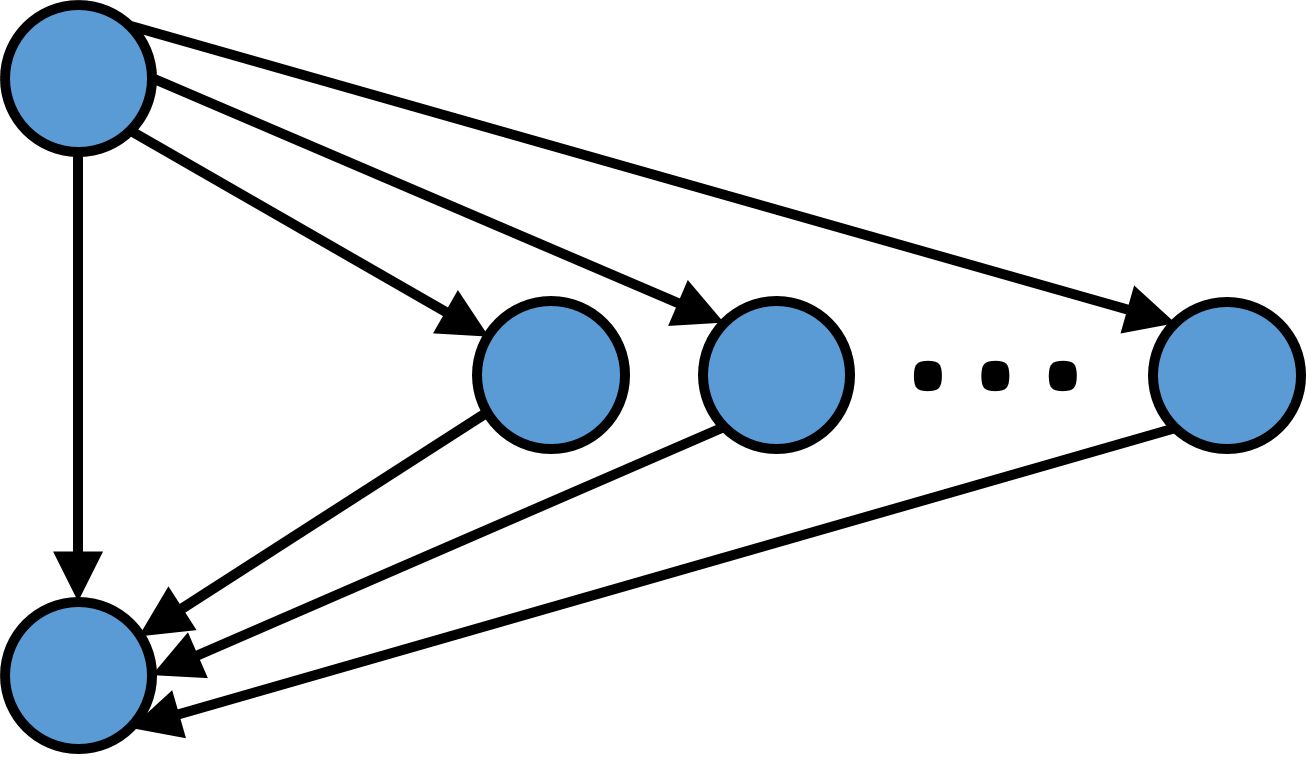
\includegraphics[width=0.6\linewidth]{Images/AT-T} \end{minipage} & $z_{AT-T} = \lambda \sum_{i = 1}^N \sum_{j = 1}^N X_{ij} \bigg[1- \bigg(1 - \frac{1}{\lambda}\bigg)^{L_2(i,j)}\bigg]$ & $L_2(i,j) = \sum_{h = 1}^N X_{ih} X_{hj}$ \\
A2P (multiple connectivity) & \begin{minipage}{.12\textwidth} \centering 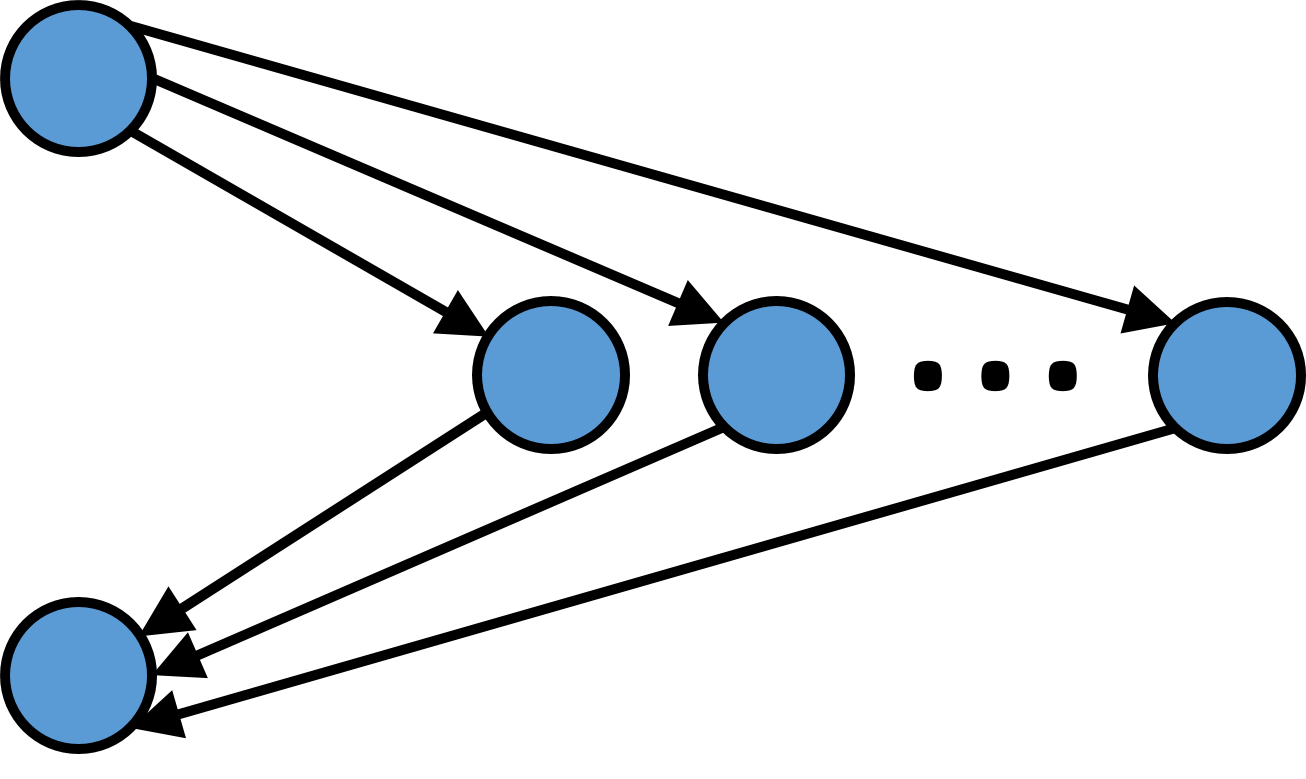
\includegraphics[width=0.6\linewidth]{Images/A2P} \end{minipage} & $z_{A2P-T} = \lambda \sum_{i < j}^N  \bigg[1- \bigg(1 - \frac{1}{\lambda}\bigg)^{L_2(i,j)}\bigg]$ & \\
Attribute sender & \begin{minipage}{.12\textwidth} \centering 
\includegraphics[width=0.4\linewidth]{Images/Sender} \end{minipage} & $z_{Sender} = \sum_{ij} u_i X_{ij}$ & \\
Attribute receiver & \begin{minipage}{.12\textwidth} \centering 
\includegraphics[width=0.4\linewidth]{Images/Receiver} \end{minipage} &  $z_{Receiver} = \sum_{ij} u_j X_{ij}$ & \\
Attribute difference & \begin{minipage}{.12\textwidth} \centering 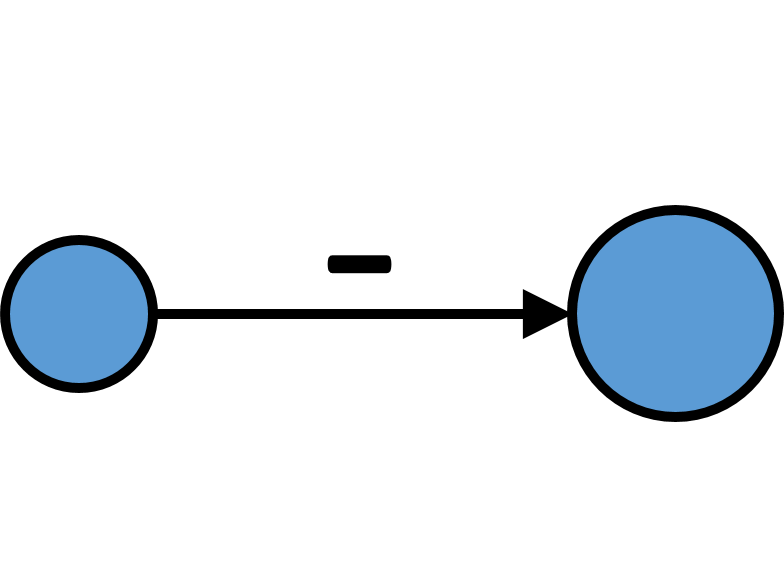
\includegraphics[width=0.4\linewidth]{Images/Difference} \end{minipage} & $z_{\mathit{Difference}} = \sum_{ij} | u_i - u_j| X_{ij}$ & \\
Attribute match & \begin{minipage}{.12\textwidth} \centering 
\includegraphics[width=0.4\linewidth]{Images/Match} \end{minipage} & $z_{Match} = \sum_{i,j} \delta_{c_i, c_j} X_{ij}$ & {\[
\delta_{c_i, c_j} =
\begin{cases}
0 & \text{if  } c_i \neq c_j, \\
1 & \text{if  } c_i = c_j. \\
\end{cases}
\]} \\
Attribute mismatch reciprocity & \begin{minipage}{.12\textwidth} \centering 
\includegraphics[width=0.4\linewidth]{Images/MisMatchReciprocity} \end{minipage} & $z_{\mathit{Mismatch\ reciprocity}} = \sum_{ij} \bigg(1 - \delta_{c_i, c_j}\bigg) X_{ij} X_{ji}$ & \\
b\textsubscript{O} (liaison role) & \begin{minipage}{.12\textwidth} \centering 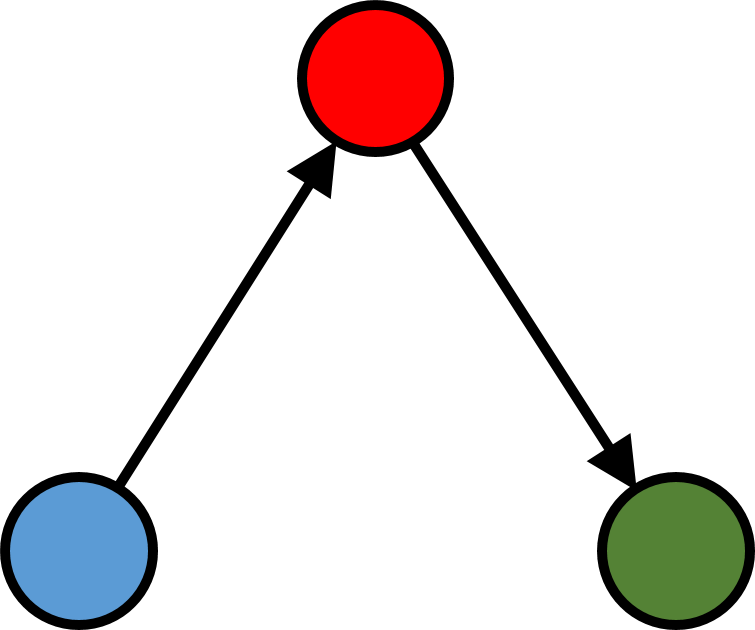
\includegraphics[width=0.4\linewidth]{Images/b_O} \end{minipage} & $z_{b_O} = \sum_{i \neq j \neq k}^N X_{ij} X_{jk} \bigg(1 - \delta_{c_i,c_j} \bigg) \bigg(1 - \delta_{c_j,c_k} \bigg)$ & \\
b\textsubscript{IO} (representative role) & \begin{minipage}{.12\textwidth} \centering 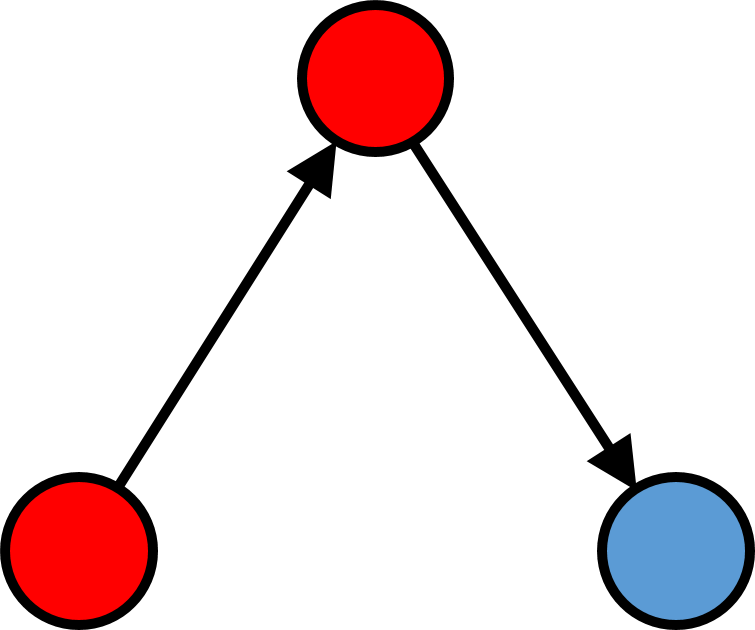
\includegraphics[width=0.4\linewidth]{Images/b_IO} \end{minipage} & $z_{b_{IO}} = \sum_{i \neq j \neq k}^N X_{ij} X_{jk} \delta_{c_i,c_j} \bigg(1 - \delta_{c_i,c_j} \bigg) \bigg(1 - \delta_{c_j,c_k} \bigg)$ & \\
b\textsubscript{OI} (gatekeeper role) & \begin{minipage}{.12\textwidth} \centering 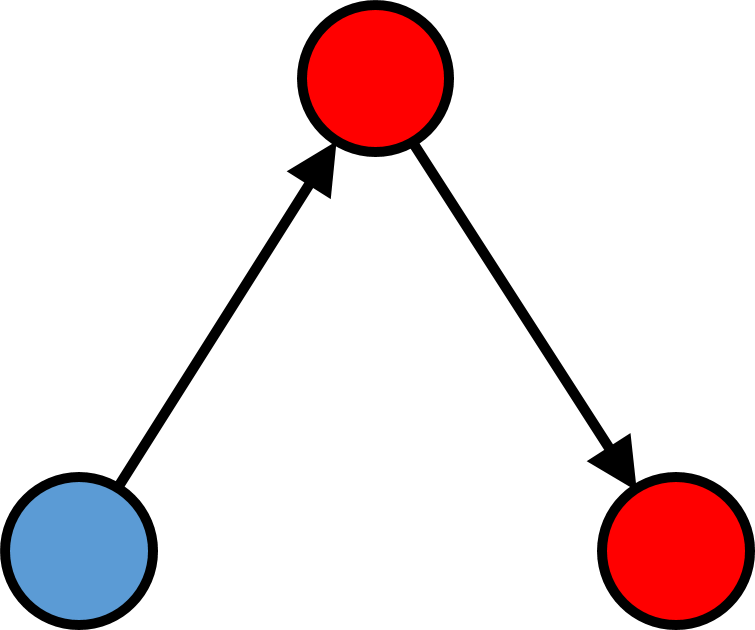
\includegraphics[width=0.4\linewidth]{Images/b_OI} \end{minipage} & $z_{b_{OI}} = \sum_{i \neq j \neq k}^N X_{ij} X_{jk} \bigg(1 - \delta_{c_i,c_j} \bigg) \delta_{c_i,c_k} \delta_{c_j,c_k}$ & \\
w\textsubscript{O} (itinerant broker) & \begin{minipage}{.12\textwidth} \centering 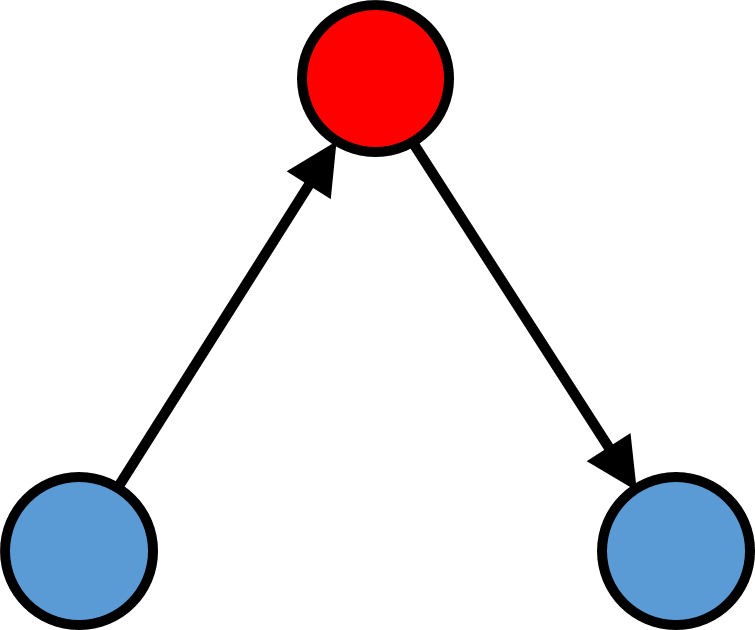
\includegraphics[width=0.4\linewidth]{Images/w_O} \end{minipage} & $z_{w_O} = \sum_{i \neq j \neq k}^N X_{ij} X_{jk} \bigg(1 - \delta_{c_i,c_j} \bigg) \delta_{c_i,c_k} \bigg(1 - \delta_{c_j,c_k} \bigg)$ & \\
w\textsubscript{I} (internal coordinator) & \begin{minipage}{.12\textwidth} \centering 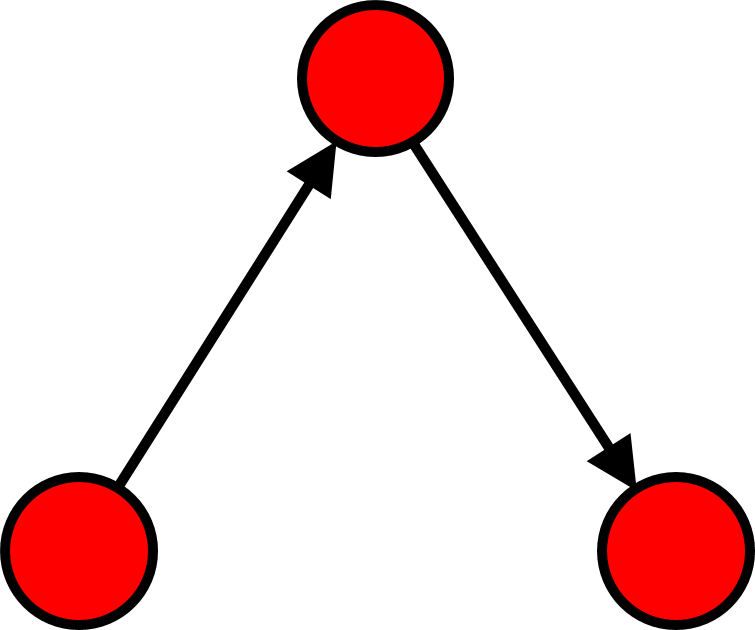
\includegraphics[width=0.4\linewidth]{Images/w_I} \end{minipage} & $z_{b_{w_I}} = \sum_{i \neq j \neq k}^N X_{ij} X_{jk} \delta_{c_i,c_j} \delta_{c_i,c_k} \delta_{c_j,c_k}$ & \\
Dyadic covariate & \begin{minipage}{.12\textwidth} \centering 
\includegraphics[width=0.4\linewidth]{Images/DyadicCovariate} \end{minipage} & $z_{Dyadic} = \sum_{i,j}^N X_{ij} Y_{ij}$ & \\
\bottomrule
\end{tabular}
\begin{tablenotes}
\footnotesize
\item[*] Refer to Table \ref{tab:ergm_params} for an explanation of each parameter.
\end{tablenotes}

\end{threeparttable}
}
\end{sidewaystable}